\chapter{Monads and Kleisli Triples}
\label{chap:monads}

\epigraph{
  La Monade, dont nous parlerons icy, n'est autre chose qu'une
  substance simple...
}{---\textcite[1]{leibniz-1714}}

In Haskell, given two types \texthaskell{a} and \texthaskell{b}, the
Cartesian product of a list \texthaskell{xs} of elements of type
\texthaskell{a} and a list \texthaskell{ys} of elements of type
\texthaskell{b} is defined to be the list of tuples
\texthaskell{(x,y)} of type \texthaskell{(a,b)} for which
\texthaskell{x} belongs to \texthaskell{xs} and \texthaskell{y}
belongs to \texthaskell{ys}, that is, using a list comprehension:
\begin{codehaskell}
cartesian :: [a] -> [b] -> [(a,b)]
cartesian xs ys = [(x,y) | x <- xs, y <- ys]
\end{codehaskell}
Or, equivalently, desugaring the list comprehension:
\begin{codehaskell}
cartesian xs ys = xs >>= \ x -> ys >>= \ y -> return (x,y)
\end{codehaskell}
This is but one simple example to show that ``a monad is often an
obvious and useful tool to help solve a problem''
\parencite[325]{osullivan-et-al-2008}, and that ``many common
programming patterns have a monadic structure''
\parencite[328]{osullivan-et-al-2008}.

In this chapter, we explore monads and Kleisli triples in order to be
able to conceptualize and better understand monads in functional
programming. As motivation, in \hask, ``we distinguish the object
\texthaskell{a} of values (of type \texthaskell{a}) from the object
\texthaskell{m a} of computations (of type \texthaskell{a}) (...). In
particular, we identify the type \texthaskell{a} with the object of
values (of type \texthaskell{a}) and obtain the object of computations
(of type \texthaskell{a}) by applying a unary type constructor
\texthaskell{m} to \texthaskell{a}. We call \texthaskell{m} a notion
of computation,'' which is just a qualitative description of a
computation \parencite[17]{moggi-1989}, ``since it abstracts away from
the type of values computations may produce''
\parencite[57--58]{moggi-1991}. There are many notions of computation.
For instance, the \texthaskell{Maybe} and \texthaskell{[]} (list) type
constructors represent the notions of partiality and nondeterminism,
respectively. Instead of studying a specific \texthaskell{m}, we focus
on monads, which describe the general properties common to such
notions of computation \parencite[58]{moggi-1991}.

In the remainder of this chapter, we define the concepts of monad and
Kleisli triple, prove their equivalence, and study both constructs in
Haskell and Agda. We should note that, terminologically,
category-theoretical monads and monads in Haskell, which actually
correspond to Kleisli triples, are not the same thing.

\section{Monads and Kleisli Triples}
\label{sec:monads}

In this section, we define the concepts of monad and Kleisli triple,
and prove their equivalence. Kleisli triples ``are easy to justify
from a computational perspective,'' but monads ``are more widely used
in (...) category theory and have the advantage of being defined only
in terms of functors and natural transformations, which make them more
suitable for abstract manipulation'' \parencite[60]{moggi-1991}.

\subsection{Monads}

First, we describe monads. Despite the fact that monads in functional
programming correspond to Kleisli triples, categorical monads are
likely more appropriate for analyzing them from the perspective of
category theory.

\begin{definition}
  \label{def:monad}

  %% \parencite[137]{maclane-1998}

  Let $\cat{C}$ be a category. A monad $\mon{T} = (\func{T},
  \nat{\eta}, \nat{\mu})$ in \cat{C} consists of an endofunctor
  $\func{T}: \cat{C} \to \cat{C}$, together with two natural
  transformations
  \begin{equation}
    \label{eq:monad-unit}
    \nat{\eta}: \func{I} \to \func{T}: \cat{C} \to \cat{C}
  \end{equation}
  and
  \begin{equation}
    \label{eq:monad-multiplication}
    \nat{\mu}: \func{T \comp T} \to \func{T}: \cat{C} \to \cat{C}
    \text{,}
  \end{equation}
  called unit and multiplication of the monad, respectively, such
  that, for all objects $a$,
  \begin{equation}
    \label{eq:monad-associativity}
    \natO{\mu}{a} \comp \natO{\mu}{\funcO{T}(a)} = \natO{\mu}{a} \comp \funcM{T}(\natO{\mu}{a})
    \text{,}
  \end{equation}
  \begin{equation}
    \label{eq:monad-unity-left}
    \natO{\mu}{a} \comp \natO{\eta}{\funcO{T}(a)} = \idO{\funcO{T}(a)}
    \text{,}
  \end{equation}
  and
  \begin{equation}
    \label{eq:monad-unity-right}
    \natO{\mu}{a} \comp \funcM{T}(\natO{\eta}{a}) = \idO{\funcO{T}(a)}
    \text{,}
  \end{equation}
  that is, the diagrams in Figures \ref{fig:monad-associativity} and
  \ref{fig:monad-unity}\footnote{We use double arrows in commutative
    diagrams to represent equality of objects.} are commutative. Since
  \nat{\eta} and \nat{\mu} are natural transformations, then, for all
  morphisms $f: a \to \funcO{T}(b)$,
  \begin{equation}
    \label{eq:monad-naturality-unit}
    \natO{\eta}{\funcO{T}(b)} \comp f = \funcM{T}(f) \comp \natO{\eta}{a}
  \end{equation}
  and
  \begin{equation}
    \label{eq:monad-naturality-multiplication}
    \natO{\mu}{\funcO{T}(b)} \comp \funcM{T}(\funcM{T}(f)) = \funcM{T}(f) \comp \natO{\mu}{a}
    \text{,}
  \end{equation}
  that is, the diagrams in Figures \ref{fig:monad-naturality-unit} and
  \ref{fig:monad-naturality-multiplication} are commutative.

  \begin{figure}[htbp]
    \begin{center}
      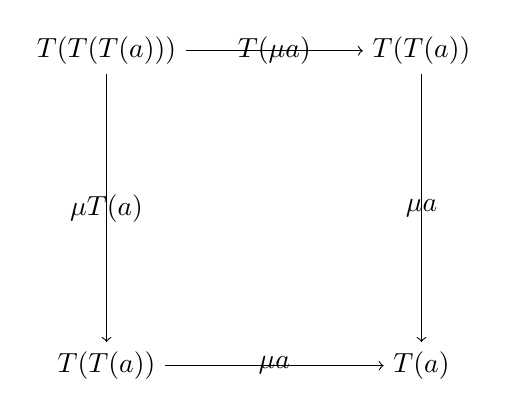
\begin{tikzpicture}[node distance=4cm]
        \node (ttt a)                  {$\funcO{T}(\funcO{T}(\funcO{T}(a)))$};
        \node (tt a1) [right of=ttt a] {$\funcO{T}(\funcO{T}(a))$};
        \node (tt a2) [below of=ttt a] {$\funcO{T}(\funcO{T}(a))$};
        \node (t a)   [right of=tt a2] {$\funcO{T}(a)$};

        \draw [->] (ttt a) to node        {$\funcM{T}(\natO{\mu}{a})$} (tt a1);
        \draw [->] (ttt a) to node [swap] {$\natO{\mu}{\funcO{T}(a)}$} (tt a2);
        \draw [->] (tt a1) to node        {$\natO{\mu}{a}$}            (t a);
        \draw [->] (tt a2) to node [swap] {$\natO{\mu}{a}$}            (t a);
      \end{tikzpicture}
    \end{center}
    \caption{Monadic associativity.}
    \label{fig:monad-associativity}
  \end{figure}

  \begin{figure}[htbp]
    \begin{center}
      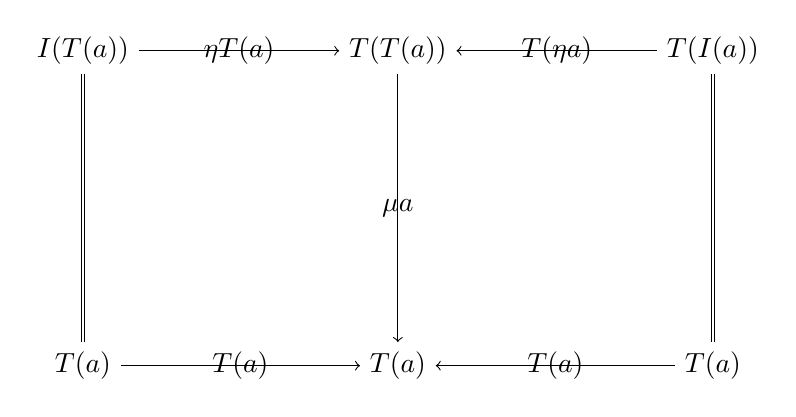
\begin{tikzpicture}[node distance=4cm]
        \node (it a)                 {$\funcO{I}(\funcO{T}(a))$};
        \node (tt a) [right of=it a] {$\funcO{T}(\funcO{T}(a))$};
        \node (ti a) [right of=tt a] {$\funcO{T}(\funcO{I}(a))$};
        \node (t a1) [below of=it a] {$\funcO{T}(a)$};
        \node (t a2) [right of=t a1] {$\funcO{T}(a)$};
        \node (t a3) [right of=t a2] {$\funcO{T}(a)$};

        \draw [->] (it a) to node        {$\natO{\eta}{\funcO{T}(a)}$} (tt a);
        \draw [->] (ti a) to node [swap] {$\funcM{T}(\natO{\eta}{a})$} (tt a);

        \draw [double] (it a) to                        (t a1);
        \draw [->]     (tt a) to node {$\natO{\mu}{a}$} (t a2);
        \draw [double] (ti a) to                        (t a3);

        \draw [->] (t a1) to node [swap] {$\idO{\funcO{T}(a)}$} (t a2);
        \draw [->] (t a3) to node        {$\idO{\funcO{T}(a)}$} (t a2);
      \end{tikzpicture}
    \end{center}
    \caption{Monadic unity.}
    \label{fig:monad-unity}
  \end{figure}

  \begin{figure}[htbp]
    \begin{center}
      \begin{tikzpicture}[node distance=4cm]
        \node (f a)                {$a$};
        \node (f b) [below of=f a] {$\funcO{T}(b)$};
        \node (g a) [right of=f a] {$\funcO{T}(a)$};
        \node (g b) [below of=g a] {$\funcO{T}(\funcO{T}(b))$};

        \draw [->] (f a) to node [swap] {$f$}            (f b);
        \draw [->] (g a) to node        {$\funcM{T}(f)$} (g b);

        \draw [->] (f a) to node        {$\natO{\eta}{a}$}            (g a);
        \draw [->] (f b) to node [swap] {$\natO{\eta}{\funcO{T}(b)}$} (g b);
      \end{tikzpicture}
    \end{center}
    \caption{Naturality of the \nat{\eta} natural transformation.}
    \label{fig:monad-naturality-unit}
  \end{figure}

  \begin{figure}[htbp]
    \begin{center}
      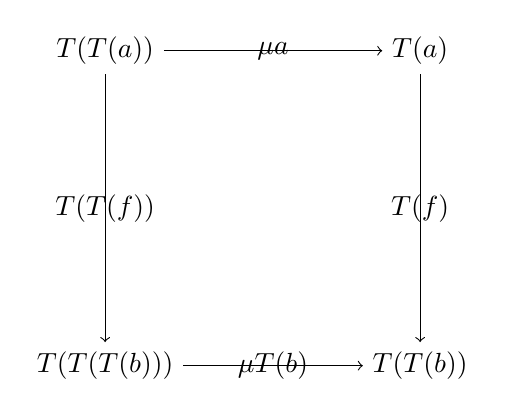
\begin{tikzpicture}[node distance=4cm]
        \node (f a)                {$\funcO{T}(\funcO{T}(a))$};
        \node (f b) [below of=f a] {$\funcO{T}(\funcO{T}(\funcO{T}(b)))$};
        \node (g a) [right of=f a] {$\funcO{T}(a)$};
        \node (g b) [below of=g a] {$\funcO{T}(\funcO{T}(b))$};

        \draw [->] (f a) to node [swap] {$\funcM{T}(\funcM{T}(f))$} (f b);
        \draw [->] (g a) to node        {$\funcM{T}(f)$}            (g b);

        \draw [->] (f a) to node        {$\natO{\mu}{a}$}            (g a);
        \draw [->] (f b) to node [swap] {$\natO{\mu}{\funcO{T}(b)}$} (g b);
      \end{tikzpicture}
    \end{center}
    \caption{Naturality of the \nat{\mu} natural transformation.}
    \label{fig:monad-naturality-multiplication}
  \end{figure}

\end{definition}

\begin{remark}
  \label{re:monad-monoid}

  Formally, the definition of a monad is like that of a monoid as
  described in Example \ref{ex:category-monoid}. Let $\mon{T} =
  (\func{T}, \nat{\eta}, \nat{\mu})$ be a monad in a category
  $\cat{C}$. The endofunctor $\func{T}$ is the set of elements of a
  monoid $M = (\func{T}, \nat{\eta}, \nat{\mu})$. The multiplication
  natural transformation, $\nat{\eta}$, is the associative binary
  operation of the monoid, and it has an identity, the unit natural
  transformation, $\nat{\mu}$. Thus, the diagram in Figure
  \ref{fig:monad-associativity} is the associative law for the monad,
  while the diagram in Figure \ref{fig:monad-unity} expresses the left
  and right unit laws \parencite[138]{maclane-1998}.

\end{remark}

As examples of monads, we consider the identity monad, which is just a
reformulation of the identity functor for a given category.

\begin{example}
  \label{ex:monad-identity}

  Let $\cat{C}$ be a category. The identity or trivial monad of
  $\cat{C}$ is $\mon{I} = (\func{I}, \id, \id)$, that is, the identity
  endofunctor (see Example \ref{ex:functor-identity}) and the identity
  mapping of $\cat{C}$. Equations \eqref{eq:monad-associativity},
  \eqref{eq:monad-unity-left}, and \eqref{eq:monad-unity-right} hold
  by \eqref{eq:category-identity}, and
  \eqref{eq:monad-naturality-unit} and
  \eqref{eq:monad-naturality-multiplication} hold because \nat{\id} is
  a natural transformation (see Example \ref{ex:natural-identity}).

\end{example}

\subsection{Kleisli Triples}

Now, we describe Kleisli triples, which ``are just an alternative
description for monads'' \parencite[60]{moggi-1991}.

\begin{definition}
  \label{def:triple}

  %% \parencite[58]{moggi-1991}

  Let $\cat{C}$ be a category. A Kleisli triple $\mon{T} = (\funcO{T},
  \nat{\eta}, \monM{T}{\underscore})$ in $\cat{C}$, where $\nat{\eta}$
  is a transformation \eqref{eq:monad-unit}, assigns to each object
  $a$ an object $\funcO{T}(a)$, and to each morphism $f: a \to
  \funcO{T}(b)$ a morphism $\monM{T}{f}: \funcO{T}(a) \to
  \funcO{T}(b)$, such that, for all morphisms $f: a \to \funcO{T}(b)$
  and $g: b \to \funcO{T}(c)$,
  \begin{equation}
    \label{eq:triple-associativity}
    \monM{T}{g} \comp \monM{T}{f} = \monM{T}{(\monM{T}{g} \comp f)}
    \text{,}
  \end{equation}
  for all morphisms $f: a \to \funcO{T}(b)$,
  \begin{equation}
    \label{eq:triple-unity-left}
    \monM{T}{f} \comp \natO{\eta}{a} = f
    \text{,}
  \end{equation}
  and, for all objects $a$,
  \begin{equation}
    \label{eq:triple-unity-right}
    \monM{T}{\natO{\eta}{a}} = \idO{\funcO{T}(a)}
    \text{,}
  \end{equation}
  that is, the diagrams in Figures \ref{fig:triple-associativity} and
  \ref{fig:triple-unity} are commutative, and
  \eqref{eq:triple-unity-right}.

  \begin{figure}[htb]
    \begin{subfigure}[b]{0.45\linewidth}
      \begin{center}
        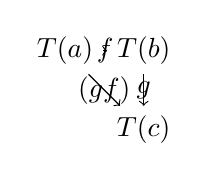
\begin{tikzpicture}
          \node (t a)                {$\funcO{T}(a)$};
          \node (t b) [right of=t a] {$\funcO{T}(b)$};
          \node (t c) [below of=t b] {$\funcO{T}(c)$};

          \draw [->] (t a) to node        {$\monM{}{f}$}                    (t b);
          \draw [->] (t a) to node [swap] {$\monM{}{(\monM{}{g} \comp f)}$} (t c);
          \draw [->] (t b) to node        {$\monM{}{g}$}                    (t c);
        \end{tikzpicture}
      \end{center}
      \caption{Kleisli triple associativity.}
      \label{fig:triple-associativity}
    \end{subfigure}
    \begin{subfigure}[b]{0.45\linewidth}
      \begin{center}
        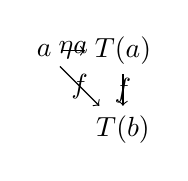
\begin{tikzpicture}
          \node (a)                  {$a$};
          \node (t a) [right of=a]   {$\funcO{T}(a)$};
          \node (t b) [below of=t a] {$\funcO{T}(b)$};

          \draw [->] (a)   to node        {$\natO{\eta}{a}$} (t a);
          \draw [->] (a)   to node [swap] {$f$}              (t b);
          \draw [->] (t a) to node        {$\monM{}{f}$}     (t b);
        \end{tikzpicture}
      \end{center}
      \caption{Kleisli triple unity.}
      \label{fig:triple-unity}
    \end{subfigure}
    \caption{Kleisli triple laws.}
  \end{figure}

\end{definition}

\begin{remark}
  \label{re:triple}

  From a computational perspective, ``$\natO{\eta}{a}$ is the
  inclusion of values into computations and $\monM{T}{f}$ is the
  extension of a function $f$ from values to computations to a
  function from computations to computations, which first evaluates a
  computation and then applies $f$ to the resulting value''
  \parencite[59]{moggi-1991}.

\end{remark}

\begin{remark}
  \label{re:monad-triple}

  Unlike the definition of a monad, a Kleisli triple does not require
  an endofunctor, just an object mapping, and its unit is not required
  to be defined as a natural transformation, just a transformation.

\end{remark}

As examples, we describe the identity or trivial monad as a Kleisli
triple.

\begin{example}
  \label{ex:triple-identity}

  Let $\cat{C}$ be a category. The identity or trivial Kleisli triple
  of $\cat{C}$ is $\mon{I} = (\funcO{I}, \id, \funcM{I})$, that is,
  the object mapping of the identity endofunctor (see Example
  \ref{ex:functor-identity}), the identity mapping, and the morphism
  mapping of the identity endofunctor of $\cat{C}$. Equation
  \eqref{eq:triple-associativity} holds by
  \eqref{eq:category-associativity}, and \eqref{eq:triple-unity-left}
  and \eqref{eq:triple-unity-right} hold by
  \eqref{eq:category-identity}. This is just an alternative
  description of the identity monad (see Example
  \ref{ex:monad-identity}).

\end{example}

\subsection{Equivalence of Monads and Kleisli Triples}

Algebraic theories in clone form \parencite[24]{manes-1976}, which we
shall refer to as monads in clone form, are yet another alternative
description for monads. \textcite[26--29]{manes-1976} thoroughly
proved the equivalence between monads and monads in clone form, and
\textcite[61]{moggi-1991} stated the equivalence between monads and
Kleisli triples, and proved it without going into details. The
following theorems demonstrate in a thorough manner that monads and
Kleisli triples are equivalent. As illustrated in Figure
\ref{fig:monad-theory-triple}, these proofs are enough for stating the
equivalence between the three alternative descriptions.

\begin{figure}[htb]
  \begin{center}
    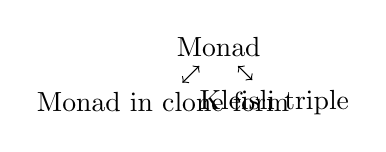
\begin{tikzpicture}
      \node (monad)                         {Monad};
      \node (theory) [below left of=monad]  {Monad in clone form};
      \node (triple) [below right of=monad] {Kleisli triple};

      \draw [<->] (monad) to (theory);
      \draw [<->] (monad) to (triple);
    \end{tikzpicture}
  \end{center}
  \caption{Equivalence of monads, monads in clone form, and Kleisli triples.}
  \label{fig:monad-theory-triple}
\end{figure}

First, we state that a Kleisli triple can be obtained from a monad.
Since monads are defined in terms of functors and natural
transformations, the following lemma is simpler than its converse.

\begin{lemma}
  \label{lem:monad-to-triple}

  %% \parencite[61]{moggi-1991}

  Let $\mon{T} = (\func{T}, \nat{\eta}, \nat{\mu})$ be a monad in a
  category $\cat{C}$. Then
  \begin{equation*}
    \mon{T} = (\funcO{T}, \nat{\eta}, \monM{}{\underscore})
    \text{,}
  \end{equation*}
  where $\funcO{T}$ is the object mapping of the endofunctor
  $\func{T}$, $\nat{\eta}$ is the underlying transformation of the
  natural transformation $\nat{\eta}$, and $\monM{}{\underscore}$
  assigns to each morphism $f : a \to \funcO{T}(b)$ a morphism
  $\monM{}{f}: \funcO{T}(a) \to \funcO{T}(b)$ defined by
  \begin{equation}
    \label{eq:monad-to-triple-extension}
    \monM{}{f} = \natO{\mu}{b} \comp \funcM{T}(f)
    \text{,}
  \end{equation}
  is a Kleisli triple in $\cat{C}$.

  \begin{proof}

    First, we prove that \eqref{eq:triple-associativity} holds:
    \begin{steps}
      \stepm{\monM{}{g} \comp \monM{}{f}}
        \eqby{\eqref{eq:monad-to-triple-extension} with $f = f$ and $f = g$}
      \stepm{\natO{\mu}{c} \comp \funcM{T}(g) \comp \natO{\mu}{b} \comp \funcM{T}(f)}
        \eqby{\eqref{eq:monad-naturality-multiplication} with $f = g$}
      \stepm{\natO{\mu}{c} \comp \natO{\mu}{\funcO{T}(c)} \comp \funcM{T}(\funcM{T}(g)) \comp \funcM{T}(f)}
        \eqby{\eqref{eq:functor-composition} with $g = \funcM{T}(g)$}
      \stepm{\natO{\mu}{c} \comp \natO{\mu}{\funcO{T}(c)} \comp \funcM{T}(\funcM{T}(g) \comp f)}
        \eqby{\eqref{eq:monad-associativity} with $a = c$}
      \stepm{\natO{\mu}{c} \comp \funcM{T}(\natO{\mu}{c}) \comp \funcM{T}(\funcM{T}(g) \comp f)}
        \eqby{\eqref{eq:functor-composition} with $f = \funcM{T}(g) \comp f$ and $g = \natO{\mu}{c}$}
      \stepm{\natO{\mu}{c} \comp \funcM{T}(\natO{\mu}{c} \comp \funcM{T}(g) \comp f)}
        \eqby{\eqref{eq:monad-to-triple-extension} with $f = g$ and $f = \monM{}{g} \comp f$}
      \stepm{\monM{}{(\monM{}{g} \comp f)}}
    \end{steps}
    Now, we prove that \eqref{eq:triple-unity-left} holds:
    \begin{steps}
      \stepm{\monM{}{f} \comp \natO{\eta}{a}}
        \eqby{\eqref{eq:monad-to-triple-extension}}
      \stepm{\natO{\mu}{b} \comp \funcM{T}(f) \comp \natO{\eta}{a}}
        \eqby{\eqref{eq:monad-naturality-unit}}
      \stepm{\natO{\mu}{b} \comp \natO{\eta}{\funcO{T}(b)} \comp f}
        \eqby{\eqref{eq:monad-unity-left} with $a = b$}
      \stepm{\idO{\funcO{T}(b)} \comp f}
        \eqby{\eqref{eq:category-identity}}
      \stepm{f}
    \end{steps}
    Finally, we prove that \eqref{eq:triple-unity-right} holds:
    \begin{steps}
      \stepm{\monM{}{\natO{\eta}{a}}}
        \eqby{\eqref{eq:monad-to-triple-extension} with $f = \natO{\eta}{a}$}
      \stepm{\natO{\mu}{a} \comp \funcM{T}(\natO{\eta}{a})}
        \eqby{\eqref{eq:monad-unity-right}}
      \stepm{\idO{\funcO{T}(a)}}
    \end{steps}

  \end{proof}

\end{lemma}

The object mapping of a Kleisli triple can be extended to define an
endofunctor, as proven in the following lemma.

\begin{proposition}
  \label{prop:triple-to-endofunctor}

  %% \parencite[61]{moggi-1991}

  Let $\cat{C}$ be a category. If $\mon{T} = (\funcO{T}, \nat{\eta},
  \monM{}{\underscore})$ is a Kleisli triple in $\cat{C}$, then
  $\func{T} = (\funcO{T}, \funcM{T})$, which assigns to each morphism
  $f: a \to b$ a morphism $\funcM{T}(f): \funcO{T}(a) \to
  \funcO{T}(b)$ defined by
  \begin{equation}
    \label{eq:triple-to-endofunctor-morphism-function}
    \funcM{T}(f) = \monM{}{(\natO{\eta}{b} \comp f)}
    \text{,}
  \end{equation}
  is an endofunctor in $\cat{C}$.

  \begin{proof}

    In the first place, we prove that \eqref{eq:functor-identity}
    holds:
    \begin{steps}
      \stepm{\funcM{T}(\idO{a})}
        \eqby{\eqref{eq:triple-to-endofunctor-morphism-function} with $f = \idO{a}$}
      \stepm{\monM{}{(\natO{\eta}{a} \comp \idO{a})}}
        \eqby{\eqref{eq:category-identity} with $f = \natO{\eta}{a}$}
      \stepm{\monM{}{\natO{\eta}{a}}}
    \end{steps}
    In the second place, we prove that \eqref{eq:functor-composition}
    holds:
    \begin{steps}
      \stepm{\funcM{T}(g \comp f)}
        \eqby{\eqref{eq:triple-to-endofunctor-morphism-function} with $f = g \comp f$}
      \stepm{\monM{}{(\natO{\eta}{c} \comp g \comp f)}}
        \eqby{\eqref{eq:triple-unity-left} with $f = \natO{\eta}{c} \comp g$}
      \stepm{\monM{}{(\monM{}{(\natO{\eta}{c} \comp g)} \comp \natO{\eta}{b} \comp f)}}
        \eqby{\eqref{eq:triple-associativity} with $f = \natO{\eta}{b} \comp f$ and $g = \natO{\eta}{c} \comp g$}
      \stepm{\monM{}{(\natO{\eta}{c} \comp g)} \comp \monM{}{(\natO{\eta}{b} \comp f)}}
        \eqby{\eqref{eq:triple-to-endofunctor-morphism-function} with $f = f$ and $f = g$}
      \stepm{\funcM{T}(g) \comp \funcM{T}(f)}
    \end{steps}

  \end{proof}

\end{proposition}

Now, since $\func{T}$ is an endofunctor, we state and prove that
$\nat{\eta}$ is a natural transformation.

\begin{proposition}
  \label{prop:triple-to-monad-unit}

  If $\mon{T} = (\funcO{T}, \nat{\eta}, \monM{}{\underscore})$ is a
  Kleisli triple in a category $\cat{C}$, then the transformation
  $\nat{\eta}$ is natural.

  \begin{proof}

    We prove that \eqref{eq:naturality} holds for $\nat{\eta}$:
    \begin{steps}
      \stepm{\natO{\eta}{\funcO{T}(b)} \comp f}
        \eqby{\eqref{eq:triple-unity-left} with $f = \natO{\eta}{\funcO{T}(b)} \comp f$}
      \stepm{\monM{}{(\natO{\eta}{\funcO{T}(b)} \comp f)} \comp \natO{\eta}{a}}
        \eqby{\eqref{eq:triple-to-endofunctor-morphism-function}}
      \stepm{\funcM{T}(f) \comp \natO{\eta}{a}}
    \end{steps}

  \end{proof}

\end{proposition}

Next, we define the multiplication of a monad given a Kleisli triple,
and prove that it is a natural transformation.

\begin{proposition}
  \label{prop:triple-to-monad-multiplication}

  %% \parencite[61]{moggi-1991}

  Let $\cat{C}$ be a category. If $\mon{T} = (\funcO{T}, \nat{\eta},
  \monM{}{\underscore})$ is a Kleisli triple in $\cat{C}$, then a
  transformation $\nat{\mu}$ which assigns to each object $a$ a
  morphism $\natO{\mu}{a}: \funcO{T}(\funcO{T}(a)) \to \funcO{T}(a)$
  defined by
  \begin{equation}
    \label{eq:triple-to-monad-multiplication}
    \natO{\mu}{a} = \monM{}{\idO{\funcO{T}(a)}}
  \end{equation}
  is a natural transformation $\nat{\mu}: \func{T} \comp \func{T} \to
  \func{T}: \cat{C} \to \cat{C}$.

  \begin{proof}

    We prove that \eqref{eq:naturality} holds for $\nat{\mu}$:
    \begin{steps}
      \stepm{\natO{\mu}{\funcO{T}(b)} \comp \funcM{T}(\funcM{T}(f))}
        \eqby{\eqref{eq:triple-to-monad-multiplication} with $a = \funcO{T}(b)$}
      \stepm{\monM{}{\idO{\funcO{T}(\funcO{T}(b))}} \comp \funcM{T}(\funcM{T}(f))}
        \eqby{\eqref{eq:triple-to-endofunctor-morphism-function}}
      \stepm{\monM{}{\idO{\funcO{T}(\funcO{T}(b))}} \comp \funcM{T}(\monM{}{(\natO{\eta}{\funcO{T}(b)} \comp f)})}
        \eqby{\eqref{eq:triple-to-endofunctor-morphism-function} with $f = \monM{}{(\natO{\eta}{\funcO{T}(b)} \comp f)}$}
      \stepm{\monM{}{\idO{\funcO{T}(\funcO{T}(b))}} \comp \monM{}{(\natO{\eta}{\funcO{T}(\funcO{T}(b))} \comp \monM{}{(\natO{\eta}{\funcO{T}(b)} \comp f)})}}
        \eqby{\eqref{eq:triple-associativity} with $f = \natO{\eta}{\funcO{T}(\funcO{T}(b))} \comp \monM{}{(\natO{\eta}{\funcO{T}(b)} \comp f)}$ and $g = \idO{\funcO{T}(\funcO{T}(b))}$}
      \stepm{\monM{}{(\monM{}{\idO{\funcO{T}(\funcO{T}(b))}} \comp \natO{\eta}{\funcO{T}(\funcO{T}(b))} \comp \monM{}{(\natO{\eta}{\funcO{T}(b)} \comp f)})}}
        \eqby{\eqref{eq:triple-unity-left} with $f = \idO{\funcO{T}(\funcO{T}(b))}$}
      \stepm{\monM{}{(\idO{\funcO{T}(\funcO{T}(b))} \comp \monM{}{(\natO{\eta}{\funcO{T}(b)} \comp f)})}}
        \eqby{\eqref{eq:category-identity} with $f = \monM{}{(\natO{\eta}{\funcO{T}(b)} \comp f)}$}
      \stepm{\monM{}{(\monM{}{(\natO{\eta}{\funcO{T}(b)} \comp f)})}}
        \eqby{\eqref{eq:category-identity} with $f = \monM{}{(\natO{\eta}{\funcO{T}(b)} \comp f)}$}
      \stepm{\monM{}{(\monM{}{(\natO{\eta}{\funcO{T}(b)} \comp f)} \comp \idO{\funcO{T}(a)})}}
        \eqby{\eqref{eq:triple-associativity} with $f = \idO{\funcO{T}(a)}$ and $g = \natO{\eta}{\funcO{T}(b)} \comp f$}
      \stepm{\monM{}{(\natO{\eta}{\funcO{T}(b)} \comp f)} \comp \monM{}{\idO{\funcO{T}(a)}}}
        \eqby{\eqref{eq:triple-to-endofunctor-morphism-function}}
      \stepm{\funcM{T}(f) \comp \monM{}{\idO{\funcO{T}(a)}}}
        \eqby{\eqref{eq:triple-to-monad-multiplication}}
      \stepm{\funcM{T}(f) \comp \natO{\mu}{a}}
    \end{steps}

  \end{proof}

\end{proposition}

Now, we state that a monad can be obtained from a Kleisli triple using
the constructions from the three lemmas above.

\begin{lemma}
  \label{lem:triple-to-monad}

  Let $\mon{T} = (\funcO{T}, \nat{\eta}, \monM{}{\underscore})$ be a
  Kleisli triple in a category $\cat{C}$. Then
  \begin{equation*}
    \mon{T} = (\func{T}, \nat{\eta}, \nat{\mu})
    \text{,}
  \end{equation*}
  where $\func{T}$ is the endofunctor in $\cat{C}$ defined by Lemma
  \ref{prop:triple-to-endofunctor}, $\nat{\eta}$ is the transformation
  \nat{\eta} regarded as a natural transformation (see Lemma
  \ref{prop:triple-to-monad-unit}), and $\nat{\mu}: \func{T} \comp
  \func{T} \to \func{T}: \cat{C} \to \cat{C}$ is the natural
  transformation defined by Lemma
  \ref{prop:triple-to-monad-multiplication}, is a monad in $\cat{C}$.

  \begin{proof}

    First, we prove that \eqref{eq:monad-associativity} holds:
    \begin{steps}
      \stepm{\natO{\mu}{a} \comp \natO{\mu}{\funcO{T}(a)}}
        \eqby{\eqref{eq:triple-to-monad-multiplication} with $a = a$ and $a = \funcO{T}(a)$}
      \stepm{\monM{}{\idO{\funcO{T}(a)}} \comp \monM{}{\idO{\funcO{T}(\funcO{T}(a))}}}
        \eqby{\eqref{eq:triple-associativity} with $f = \idO{\funcO{T}(\funcO{T}(a))}$ and $g = \idO{\funcO{T}(a)}$}
      \stepm{\monM{}{(\monM{}{\idO{\funcO{T}(a)}} \comp \idO{\funcO{T}(\funcO{T}(a))})}}
        \eqby{\eqref{eq:category-identity} with $f = \monM{}{\idO{\funcO{T}(a)}}$}
      \stepm{\monM{}{(\monM{}{\idO{\funcO{T}(a)}})}}
        \eqby{\eqref{eq:category-identity} with $f = \monM{}{\idO{\funcO{T}(a)}}$}
      \stepm{\monM{}{(\idO{\funcO{T}(a)} \comp \monM{}{\idO{\funcO{T}(a)}})}}
        \eqby{\eqref{eq:triple-unity-left} with $f = \idO{\funcO{T}(a)}$}
      \stepm{\monM{}{(\monM{}{\idO{\funcO{T}(a)}} \comp \natO{\eta}{\funcO{T}(a)} \comp \monM{}{\idO{\funcO{T}(a)}})}}
        \eqby{\eqref{eq:triple-associativity} with $f = \natO{\eta}{\funcO{T}(a)} \comp \monM{}{\idO{\funcO{T}(a)}}$ and $g = \idO{\funcO{T}(a)}$}
      \stepm{\monM{}{\idO{\funcO{T}(a)}} \comp \monM{}{(\natO{\eta}{\funcO{T}(a)} \comp \monM{}{\idO{\funcO{T}(a)}})}}
        \eqby{\eqref{eq:triple-to-monad-multiplication}}
      \stepm{\natO{\mu}{a} \comp \monM{}{(\natO{\eta}{\funcO{T}(a)} \comp \natO{\mu}{a})}}
        \eqby{\eqref{eq:triple-to-endofunctor-morphism-function} with $f = \natO{\mu}{a}$}
      \stepm{\natO{\mu}{a} \comp \funcM{T}(\natO{\mu}{a})}
    \end{steps}
    Now, we prove that \eqref{eq:monad-unity-left} holds:
    \begin{steps}
      \stepm{\natO{\mu}{a} \comp \natO{\eta}{\funcO{T}(a)}}
        \eqby{\eqref{eq:triple-to-monad-multiplication}}
      \stepm{\monM{}{\idO{\funcO{T}(a)}} \comp \natO{\eta}{\funcO{T}(a)}}
        \eqby{\eqref{eq:triple-unity-left} with $f = \idO{\funcO{T}(a)}$}
      \stepm{\idO{\funcO{T}(a)}}
    \end{steps}
    Finally, we prove that \eqref{eq:monad-unity-right} holds:
    \begin{steps}
      \stepm{\natO{\mu}{a} \comp \funcM{T}(\natO{\eta}{a})}
        \eqby{\eqref{eq:triple-to-monad-multiplication}}
      \stepm{\monM{}{\idO{\funcO{T}(a)}} \comp \funcM{T}(\natO{\eta}{a})}
        \eqby{\eqref{eq:triple-to-endofunctor-morphism-function} with $f = \natO{\eta}{a}$}
      \stepm{\monM{}{\idO{\funcO{T}(a)}} \comp \monM{}{(\natO{\eta}{\funcO{T}(a)} \comp \natO{\eta}{a})}}
        \eqby{\eqref{eq:triple-associativity} with $f = \natO{\eta}{\funcO{T}(a)} \comp \natO{\eta}{a}$ and $g = \idO{\funcO{T}(a)}$}
      \stepm{\monM{}{(\monM{}{\idO{\funcO{T}(a)}} \comp \natO{\eta}{\funcO{T}(a)} \comp \natO{\eta}{a})}}
        \eqby{\eqref{eq:triple-unity-left} with $f = \idO{\funcO{T}(a)}$}
      \stepm{\monM{}{(\idO{\funcO{T}(a)} \comp \natO{\eta}{a})}}
        \eqby{\eqref{eq:category-identity} with $f = \natO{\eta}{a}$}
      \stepm{\monM{}{\natO{\eta}{a}}}
        \eqby{\eqref{eq:triple-unity-right}}
      \stepm{\idO{\funcO{T}(a)}}
    \end{steps}

  \end{proof}

\end{lemma}

Finally, in the following theorem, we prove that monads and Kleisli
triples are equivalent.

\begin{theorem}
  \label{the:monad-triple}

  Monads and Kleisli triples are coextensive.

  \begin{proof}

    The correspondence between monads and Kleisli triples is given by
    Lemma \ref{lem:monad-to-triple}, which proves that a Kleisli
    triple can be derived from a monad, and Lemma
    \ref{lem:triple-to-monad}, which proves that a monad can be
    derived from a Kleisli triple.

  \end{proof}

\end{theorem}

\section{Monads and Kleisli Triples in Haskell}
\label{sec:monads-haskell}

When discussing monads, there are three possibilities: monads (in
monoid form), Kleisli triples (monads in extension form), and monads
in clone form. Kleisli triples are easier to justify from a
computational point of view and correspond to the representation that
is found in functional programming languages like Haskell and the Agda
standard library. On the other hand, monads have some mathematical
advantages and are more intuitive in some cases. In this section, we
describe both representations in Haskell.

\subsection{Monads in Haskell}

In \hask, a monad consists of an endofunctor, together with two
parametrically polymorphic functions, as follows\footnote{Note that
  this is not a standard Haskell type class.}:
\begin{codehaskell}
class Functor m => Monad' m where
  return :: a -> m a
  join   :: m (m a) -> m a
\end{codehaskell}
The endofunctor \texthaskell{m} corresponds to the endofunctor
$\func{T}$ of a monad, and the \texthaskell{return} and
\texthaskell{join} functions correspond to the unit and multiplication
natural transformations of a monad, $\nat{\eta}$ and $\nat{\mu}$,
respectively. Equation \eqref{eq:monad-associativity}, monadic
associativity, becomes the commutativity of the diagram in Figure
\ref{fig:monad-associativity-haskell}:
\begin{codehaskell}
join . join = join . fmap join
\end{codehaskell}
Equations \eqref{eq:monad-unity-left} and
\eqref{eq:monad-unity-right}, monadic unity, become the commutativity
of the diagram in Figure \ref{fig:monad-unity-haskell}:
\begin{codehaskell}
join . return = id = join . fmap return
\end{codehaskell}

\begin{figure}[htb]
  \begin{center}
    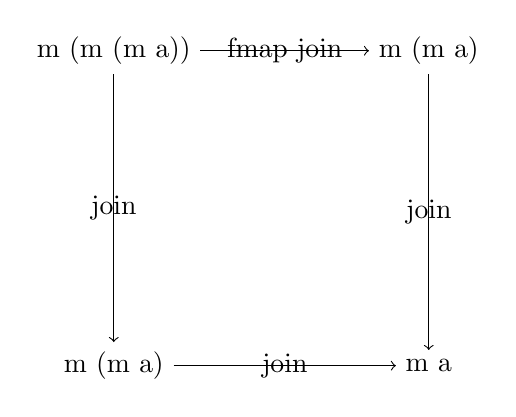
\begin{tikzpicture}[node distance=4cm]
      \node (ttt a)                  {\texthaskell{m (m (m a))}};
      \node (tt a1) [right of=ttt a] {\texthaskell{m (m a)}};
      \node (tt a2) [below of=ttt a] {\texthaskell{m (m a)}};
      \node (t a)   [right of=tt a2] {\texthaskell{m a}};

      \draw [->] (ttt a) to node        {\texthaskell{fmap join}} (tt a1);
      \draw [->] (ttt a) to node [swap] {\texthaskell{join}}      (tt a2);
      \draw [->] (tt a1) to node        {\texthaskell{join}}      (t a);
      \draw [->] (tt a2) to node [swap] {\texthaskell{join}}      (t a);
    \end{tikzpicture}
  \end{center}
  \caption{Monadic associativity in \hask.}
  \label{fig:monad-associativity-haskell}
\end{figure}

\begin{figure}[htb]
  \begin{center}
    \begin{tikzpicture}[node distance=4cm]
      \node (it a)                 {\texthaskell{m a}};
      \node (tt a) [right of=it a] {\texthaskell{m (m a)}};
      \node (ti a) [right of=tt a] {\texthaskell{m a}};
      \node (t a2) [right of=t a1] {\texthaskell{m a}};


      \draw [->] (it a) to node        {\texthaskell{return}}      (tt a);
      \draw [->] (ti a) to node [swap] {\texthaskell{fmap return}} (tt a);

      \draw [->]     (tt a) to node {\texthaskell{join}} (t a2);

      \draw [->] (it a) to node [swap] {\texthaskell{id}} (t a2);
      \draw [->] (ti a) to node        {\texthaskell{id}} (t a2);
    \end{tikzpicture}
  \end{center}
  \caption{Monadic unity in \hask.}
  \label{fig:monad-unity-haskell}
\end{figure}

In addition, by parametricity (see Section
\ref{sec:naturals-haskell}), the naturality of the unit natural
transformation, \eqref{eq:monad-naturality-unit}, becomes the free
theorem for the \texthaskell{return} function, that is, for all
functions \texthaskell{f :: a -> m b}:
\begin{codehaskell}
return . f = fmap f . return
\end{codehaskell}
Similarly, the naturality of the multiplication natural
transformation, \eqref{eq:monad-naturality-multiplication}, becomes
the free theorem for the \texthaskell{join} function, that is:
\begin{codehaskell}
join . fmap (fmap f) = fmap f . join
\end{codehaskell}

As examples, we consider the identity or trivial monad, which is an
intuitive way of learning to use the \texthaskell{Monad'} type class,
and two of the most common monads in Haskell, \texthaskell{Maybe} and
\texthaskell{[]} (list).

\begin{example}
  \label{ex:monad-identity-haskell}

  In \hask, the \texthaskell{Identity} or trivial monad, which uses
  the identity endofunctor (see Example
  \ref{ex:functor-identity-haskell}), is defined as
  follows\footnote{Using the \texthaskell{InstanceSigs} language
    option.}:
  \begin{codehaskell}
instance Monad' Identity where
  return :: a -> Identity a
  return = Identity

  join :: Identity (Identity a) -> Identity a
  join (Identity mx) = mx
  \end{codehaskell}
  This instance satisfies the monad laws, as proved in Example
  \ref{ex:monad-identity}.

\end{example}

\begin{example}
  \label{ex:monad-maybe-haskell}

  In \hask, the \texthaskell{Maybe} monad, which uses the
  \texthaskell{Maybe} endofunctor (see Example
  \ref{ex:functor-maybe-haskell}), is defined as follows:
  \begin{codehaskell}
instance Monad' Maybe where
  return :: a -> Maybe a
  return = Just

  join :: Maybe (Maybe a) -> Maybe a
  join Nothing   = Nothing
  join (Just mx) = mx
  \end{codehaskell}
  Let us see that this instance satisfies the monad laws. First, we
  prove that \eqref{eq:monad-associativity} holds:

  \vspace{1em}
  \caseh{Nothing}
  \begin{steps}
    \steph{(join . join) Nothing}
      \eqbydefh{(.)}
    \steph{join (join Nothing)}
      \eqbydefh{join}
    \steph{join Nothing}
      \eqbydefh{fmap}
    \steph{join (fmap join Nothing)}
      \eqbydefh{(.)}
    \steph{(join . fmap join) Nothing}
  \end{steps}
  \caseh{(Just mmx)}
  \begin{steps}
    \steph{(join . join) (Just mmx)}
      \eqbydefh{(.)}
    \steph{join (join (Just mmx))}
      \eqbydefh{join}
    \steph{join mmx}
      \eqbydefh{join}
    \steph{join (Just (join mmx))}
      \eqbydefh{fmap}
    \steph{join (fmap join (Just mmx))}
      \eqbydefh{(.)}
    \steph{(join . fmap join) (Just mmx)}
  \end{steps}
  Now, we prove that \eqref{eq:monad-unity-left} holds:
  \begin{steps}
    \steph{(join . return) mx}
      \eqbydef{\texthaskell{(.)}}
    \steph{join (return mx)}
      \eqbydef{\texthaskell{return}}
    \steph{join (Just mx)}
      \eqbydef{\texthaskell{join}}
    \steph{mx}
      \eqbydef{\texthaskell{id}}
    \steph{id mx}
  \end{steps}
  Finally, we prove that \eqref{eq:monad-unity-right} holds:

  \vspace{1em}
  \caseh{Nothing}
  \begin{steps}
    \steph{(join . fmap return) Nothing}
      \eqbydefh{(.)}
    \steph{join (fmap return Nothing)}
      \eqbydefh{fmap}
    \steph{join Nothing}
      \eqbydefh{join}
    \steph{Nothing}
      \eqbydefh{id}
    \steph{id Nothing}
  \end{steps}
  \caseh{(Just x)}
  \begin{steps}
    \steph{(join . fmap return) (Just x)}
      \eqbydefh{(.)}
    \steph{join (fmap return (Just x))}
      \eqbydefh{fmap}
    \steph{join (Just (return x))}
      \eqbydefh{join}
    \steph{return x}
      \eqbydefh{return}
    \steph{Just x}
      \eqbydefh{id}
    \steph{id (Just x)}
  \end{steps}

\end{example}

\begin{example}
  \label{ex:monad-list-haskell}

  In \hask, the list monad, which uses the list endofunctor (see
  Example \ref{ex:functor-list-haskell}), is declared as follows:
  \begin{codehaskell}
instance Monad' [] where
  return :: a -> [a]
  return x = [x]

  join :: [[a]] -> [a]
  join = concat
  \end{codehaskell}
  The \texthaskell{concat} function is defined as follows:
  \begin{codehaskell}
concat :: [[a]] -> [a]
concat []       = []
concat (xs:xss) = xs ++ concat xss

(++) :: [a] -> [a] -> [a]
[]     ++ ys = ys
(x:xs) ++ ys = x : xs ++ ys
  \end{codehaskell}
  Let us see that this instance satisfies the monad laws. In the first
  place, we prove, by induction, that \eqref{eq:monad-associativity}
  holds:

  \vspace{1em}
  \caseh{[]}
  \begin{steps}
    \steph{(join . join) []}
      \eqbydefsh{(.)}{join}
    \steph{concat (concat [])}
      \eqbydefh{concat}
    \steph{concat []}
      \eqbydefh{fmap}
    \steph{concat (fmap concat [])}
      \eqbydefsh{(.)}{join}
    \steph{(join . fmap join) []}
  \end{steps}
  \caseh{(xss:xsss)}
  \begin{steps}
    \steph{(join . join) (xss:xsss)}
      \eqbydefsh{(.)}{join}
    \steph{concat (concat (xss:xsss))}
      \eqbydefh{concat}
    \steph{concat (xss ++ concat xsss)}
      \eqtext{see below}
    \steph{concat xss ++ concat (concat xsss)}
      \eqbyih
    \steph{concat xss ++ concat (fmap concat xsss)}
      \eqbydefh{concat}
    \steph{concat (concat xss : fmap concat xsss)}
      \eqbydefh{fmap}
    \steph{concat (fmap concat (xss:xsss))}
      \eqbydefsh{(.)}{join}
    \steph{(join . fmap join) (xss:xsss)}
  \end{steps}
  In this proof, we use the fact that \texthaskell{concat} distributes
  over \texthaskell{(++)}:
  \begin{codehaskell}
concat (xss ++ yss) = concat xss ++ concat yss
  \end{codehaskell}
  We shall not prove this property, which could be done by induction
  on \texthaskell{xss}. Now, we prove that \eqref{eq:monad-unity-left}
  holds:
  \begin{steps}
    \steph{(join . return) xs}
      \eqbydefsh{(.)}{join}
    \steph{concat (return xs)}
      \eqbydefh{return}
    \steph{concat [xs]}
      \eqbydefh{concat}
    \steph{xs}
      \eqbydefh{id}
    \steph{id xs}
  \end{steps}
  Finally, we prove, by induction, that \eqref{eq:monad-unity-right}
  holds:

  \vspace{1em}
  \caseh{[]}
  \begin{steps}
    \steph{(join . fmap return) []}
      \eqbydefsh{(.)}{join}
    \steph{concat (fmap return [])}
      \eqbydefh{fmap}
    \steph{concat []}
      \eqbydefh{concat}
    \steph{[]}
      \eqbydefh{id}
    \steph{id []}
  \end{steps}
  \caseh{(x:xs)}
  \begin{steps}
    \steph{(join . fmap return) (x:xs)}
      \eqbydefsh{(.)}{join}
    \steph{concat (fmap return (x:xs))}
      \eqbydefh{fmap}
    \steph{concat (return x : fmap return xs)}
      \eqbydefh{concat}
    \steph{return x ++ concat (fmap return xs)}
      \eqbyih
    \steph{return x ++ id xs}
      \eqbydefsh{return}{id}
    \steph{[x] ++ xs}
      \eqbydefh{(++)}
    \steph{(x:xs)}
      \eqbydefh{id}
    \steph{id (x:xs)}
  \end{steps}

\end{example}

\subsection{Kleisli Triples in Haskell}

In \hask, a Kleisli triple consists of a type constructor, and two
functions, as follows\footnote{Note that this is not the standard
  Haskell \texthaskell{Monad} type class.}:
\begin{codehaskell}
class Monad'' m where
  return :: a -> m a
  bind   :: (a -> m b) -> m a -> m b
\end{codehaskell}
The type constructor \texthaskell{m} corresponds to the object mapping
$\funcO{T}$ of a Kleisli triple, and the \texthaskell{return} and
\texthaskell{bind} functions correspond to the unit natural
transformation and the extension mapping of a Kleisli triple,
$\nat{\eta}$ and $\monM{T}{\underscore}$, respectively. Equation
\eqref{eq:triple-associativity}, Kleisli triple associativity, becomes
the commutativity of the diagram in Figure
\ref{fig:triple-associativity-haskell}:
\begin{codehaskell}
bind g . bind f = bind (bind g . f)
\end{codehaskell}
Equation \eqref{eq:triple-unity-left}, Kleisli triple left-unity, is
the commutativity of the diagram in Figure
\ref{fig:triple-unity-haskell}:
\begin{codehaskell}
bind f . return = f
\end{codehaskell}
And \eqref{eq:triple-unity-right}, Kleisli triple right-unity,
becomes:
\begin{codehaskell}
bind return = id
\end{codehaskell}

\begin{figure}[htb]
  \begin{center}
    \begin{subfigure}[b]{0.45\linewidth}
      \begin{center}
        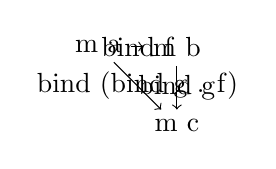
\begin{tikzpicture}
          \node (t a)                {\texthaskell{m a}};
          \node (t b) [right of=t a] {\texthaskell{m b}};
          \node (t c) [below of=t b] {\texthaskell{m c}};

          \draw [->] (t a) to node        {\texthaskell{bind f}}            (t b);
          \draw [->] (t a) to node [swap] {\texthaskell{bind (bind g . f)}} (t c);
          \draw [->] (t b) to node        {\texthaskell{bind g}}            (t c);
        \end{tikzpicture}
      \end{center}
      \caption{Kleisli triple associativity.}
      \label{fig:triple-associativity-haskell}
    \end{subfigure}
    \begin{subfigure}[b]{0.45\linewidth}
      \begin{center}
        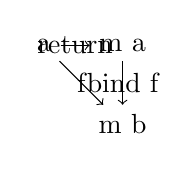
\begin{tikzpicture}
          \node (a)                  {\texthaskell{a}};
          \node (t a) [right of=a]   {\texthaskell{m a}};
          \node (t b) [below of=t a] {\texthaskell{m b}};

          \draw [->] (a)   to node        {\texthaskell{return}} (t a);
          \draw [->] (a)   to node [swap] {\texthaskell{f}}      (t b);
          \draw [->] (t a) to node        {\texthaskell{bind f}} (t b);
        \end{tikzpicture}
      \end{center}
      \caption{Kleisli triple unity.}
      \label{fig:triple-unity-haskell}
    \end{subfigure}
  \end{center}
  \caption{Kleisli triple laws in \hask.}
\end{figure}

\begin{remark}
  \label{re:triple-standard}

  Our \texthaskell{Monad''} type class corresponds to the minimal
  declaration of the standard Haskell \texthaskell{Monad} type class,
  which is not defined in terms of \texthaskell{bind}:
  \begin{codehaskell}
class Monad m where
  return :: a -> m a
  (>>=)  :: m a -> (a -> m b) -> m b

  (>>)   :: m a -> m b -> m b
  m >> k = m >>= \_ -> k

  fail   :: String -> m a
  fail = error
  \end{codehaskell}
  Given a monad with a \texthaskell{bind} function, we can get
  \texthaskell{(>>=)} as follows:
  \begin{codehaskell}
(>>=) :: Monad'' m => m a -> (a -> m b) -> m b
mx >>= f = bind f mx
  \end{codehaskell}
  In terms of standard Haskell, the \texthaskell{bind} function is
  \texthaskell{(<<=)}, which is the same as \texthaskell{(>>=)}, but
  with the arguments interchanged. Now, let us rewrite the
  \texthaskell{Monad''} laws using \texthaskell{(>>=)}. In the first
  place, since
  \begin{steps}
    \steph{(bind g . bind f) mx}
      \eqbydefh{(.)}
    \steph{bind g (bind f mx)}
      \eqbydefh{(>>=)}
    \steph{(bind f mx) >>= g}
      \eqbydefh{(>>=)}
    \steph{(mx >>= f) >>= g}
  \end{steps}
  and
  \begin{steps}
    \steph{bind (bind g . f) mx}
      \eqbydefh{(>>=)}
    \steph{mx >>= (bind g . f)}
      \eqbydefh{(.)}
    \steph{mx >>= (\textbackslash x -> bind g (f x))}
      \eqbydefh{(>>=)}
    \steph{mx >>= (\textbackslash x -> f x >>= g)}
  \end{steps}
  Kleisli triple associativity becomes
  \begin{codehaskell}
(mx >>= f) >>= g = mx >>= (\ x -> f x >>= g)
  \end{codehaskell}
  In the second place, since
  \begin{steps}
    \steph{(bind f . return) x}
      \eqbydefh{(.)}
    \steph{bind f (return x)}
      \eqbydefh{(>>=)}
    \steph{return x >>= f}
  \end{steps}
  Kleisli triple left-unity becomes
  \begin{codehaskell}
return x >>= f = f x
  \end{codehaskell}
  Finally, since
  \begin{steps}
    \steph{bind return mx}
      \eqbydefh{(>>=)}
    \steph{mx >>= return}
  \end{steps}
  Kleisli triple right-unity becomes
  \begin{codehaskell}
mx >>= return = mx
  \end{codehaskell}

  Even though our \texthaskell{Monad''} type class corresponds just to
  \texthaskell{Monad} with \texthaskell{return} and
  \texthaskell{(>>=)}, it is worth mentioning the \texthaskell{(>>)}
  and \texthaskell{fail} functions, neither of which are part of the
  mathematical definition of a Kleisli triple. In the first place,
  ``\texthaskell{(>>)} is a specialized version of
  \texthaskell{(>>=)}'' \parencite[30]{yorgey-2009}. In the second
  place, the \texthaskell{fail} function is a hack used by Haskell to
  enable failure in a \texthaskell{do} expression, which is a special
  syntactic construct for \texthaskell{Monad}
  \parencites[273]{lipovaca-2011}[88]{peytonjones-2003}[30]{yorgey-2009}.
  Besides, the \texthaskell{error} function is closely related to
  \texthaskell{undefined}\footnote{See \parencite[§
      3.1]{peytonjones-2003}.}, which we discussed in
  Convention~\ref{con:hask}.

\end{remark}

As examples, we consider the \texthaskell{Identity},
\texthaskell{Maybe}, and \texthaskell{[]} monads as Kleisli triples.

\begin{example}
  \label{ex:triple-identity-haskell}

  In \hask, the \texthaskell{Identity} or trivial Kleisli triple is
  defined as follows:
  \begin{codehaskell}
instance Monad'' Identity where
  return :: a -> Identity a
  return = Identity

  bind :: (a -> Identity b) -> Identity a -> Identity b
  bind f (Identity x) = f x
  \end{codehaskell}
  This instance satisfies the Kleisli triple laws, as proved in
  Example \ref{ex:triple-identity}.

\end{example}

\begin{example}
  \label{ex:triple-maybe-haskell}

  In \hask, the \texthaskell{Maybe} Kleisli triple is defined as
  follows:
  \begin{codehaskell}
instance Monad'' Maybe where
  return :: a -> Maybe a
  return = Just

  bind :: (a -> Maybe b) -> Maybe a -> Maybe b
  bind _ Nothing  = Nothing
  bind f (Just x) = f x
  \end{codehaskell}
  Let us see that this instance satisfies the Kleisli triple laws. We
  prove that \eqref{eq:triple-associativity} holds:

  \vspace{1em}
  \caseh{Nothing}
  \begin{steps}
    \steph{bind return Nothing}
      \eqbydefh{bind}
    \steph{Nothing}
      \eqbydefh{id}
    \steph{id Nothing}
  \end{steps}
  \caseh{(Just x)}
  \begin{steps}
    \steph{bind return (Just x)}
      \eqbydefh{return}
    \steph{return x}
      \eqbydefh{return}
    \steph{Just x}
      \eqbydefh{id}
    \steph{id (Just x)}
  \end{steps}
  Now, we prove that \eqref{eq:triple-unity-left} holds:
  \begin{steps}
    \steph{(bind f . return) x}
      \eqbydefh{(.)}
    \steph{bind f (return x)}
      \eqbydefh{return}
    \steph{bind f (Just x)}
      \eqbydefh{bind}
    \steph{f x}
  \end{steps}
  Finally, we prove that \eqref{eq:triple-unity-right} holds:

  \vspace{1em}
  \caseh{Nothing}
  \begin{steps}
    \steph{(bind g . bind f) Nothing}
      \eqbydefh{(.)}
    \steph{bind g (bind f Nothing)}
      \eqbydefh{bind}
    \steph{bind g Nothing}
      \eqbydefh{bind}
    \steph{Nothing}
      \eqbydefh{bind}
    \steph{bind (bind g . f) Nothing}
  \end{steps}
  \caseh{(Just x)}
  \begin{steps}
    \steph{(bind g . bind f) (Just x)}
      \eqbydefh{(.)}
    \steph{bind g (bind f (Just x))}
      \eqbydefh{bind}
    \steph{bind g (f x)}
      \eqbydefh{(.)}
    \steph{(bind g . f) x}
      \eqbydefh{bind}
    \steph{bind (bind g . f) (Just x)}
  \end{steps}

\end{example}

\begin{example}
  \label{ex:triple-list-haskell}

  In \hask, the \texthaskell{[]} (list) Kleisli triple is declared as
  follows:
  \begin{codehaskell}
instance Monad'' [] where
  return :: a -> [a]
  return x = [x]

  bind :: (a -> [b]) -> [a] -> [b]
  bind f xs = concat (map f xs)
  \end{codehaskell}
  We shall not prove that this instance satisfies the Kleisli triple
  laws. Since we have already proved that the list monad satisfies the
  monad laws (see Example \ref{ex:monad-list-haskell}) and that both
  representations are coextensive, we know that this instance does
  satisfy the Kleisli triple laws.

\end{example}

\subsection{Equivalence of Monads and Kleisli Triples in Haskell}

We have already proved that monads and Kleisli triples are equivalent.
In this subsection, we shall see their correspondence in terms of
Haskell. First, let us see that a \texthaskell{Monad''} (and a
\texthaskell{Monad}) can be obtained from a \texthaskell{Monad'},
which we demonstrated in Lemma \ref{lem:monad-to-triple}:
\begin{codehaskell}
bind :: Monad' m => (a -> m b) -> m a -> m b
bind f mx = join (fmap f mx)

(>>=) :: Monad' m => m a -> (a -> m b) -> m b
mx >>= f = join (fmap f mx)
\end{codehaskell}

Second, let us see that a \texthaskell{Monad'} can be obtained from a
\texthaskell{Monad''} (and from a \texthaskell{Monad}). The type
constructor of a \texthaskell{Monad''} can be extended to define an
endofunctor, which we showed in Lemma
\ref{prop:triple-to-endofunctor}:
\begin{codehaskell}
fmap :: Monad'' m => (a -> b) -> m a -> m b
fmap f mx = bind (return . f) mx

liftM :: Monad m => (a -> b) -> m a -> m b
liftM f m x = mx >>= (return . f)
\end{codehaskell}
This definition of \texthaskell{fmap} is just
\eqref{eq:triple-to-endofunctor-morphism-function}. Finally, the
\texthaskell{bind} function of a \texthaskell{Monad''} can be used to
define the \texthaskell{join} function of a \texthaskell{Monad'},
which corresponds to Lemma \ref{prop:triple-to-monad-multiplication}
or \eqref{eq:triple-to-monad-multiplication}:
\begin{codehaskell}
join' :: Monad'' m => m (m a) -> m a
join' mmx = bind id mmx

join :: Monad m => m (m a) -> m a
join mmx = mmx >>= id
\end{codehaskell}

\begin{remark}
  \label{re:monad-bind}

  In \parencite{kmett-2014}, there is a definition of bindable
  functors (that is, monads without \texthaskell{return}) which
  includes both \texthaskell{bind} and \texthaskell{join}. Thus, yet
  another type class declaration for monads and Kleisli triples is:
  \begin{codehaskell}
class Functor m => Monad''' m where
  return :: a -> m a

  bind :: (a -> m b) -> m a -> m b
  bind f = join . fmap f

  join :: m (m a) -> m a
  join = bind id
  \end{codehaskell}

\end{remark}

\section{Monads and Kleisli Triples in Agda}
\label{sec:monads-agda}

In this section, we describe monads and Kleisli triples in Agda. Since
we have already described both representations in category theory and
Haskell, we shall not go into a lot of detail here.

\subsection{Monads in Agda}

Monads in \agda are defined by the \textagda{Monad'} record, which can
be found in the module \module{Abel.Category.Monad}. This declaration
includes the monad laws, even naturalities, and the \textagda{bind}
function, which corresponds to the fact that a Kleisli triple can be
obtained from a monad.
\begin{codeagda}
record Monad' {M : Set → Set} (functor : Functor M) : Set₁ where

  constructor mkMonad'

  open Functor functor using (fmap)

  field

    return : {A : Set} → A → M A

    join   : {A : Set} → M (M A) → M A

    associativity : {A : Set} (mmmx : M (M (M A))) →
                    join (join mmmx) ≡ join (fmap join mmmx)

    unity-left    : {A : Set} (mx : M A) → join (return mx) ≡ mx

    unity-right   : {A : Set} (mx : M A) → join (fmap return mx) ≡ mx

    naturality-return : {A B : Set} {f : A → M B} (x : A) →
                        return (f x) ≡ fmap f (return x)

    naturality-join   : {A B : Set} {f : A → M B} (mmx : M (M A)) →
                        join (fmap (fmap f) mmx) ≡ fmap f (join mmx)

  bind : {A B : Set} → (A → M B) → M A → M B
  bind f = join ∘ fmap f
\end{codeagda}

As examples, we consider all the monads from Section
\ref{sec:monads-haskell}, that is, the \textagda{Identity},
\textagda{Maybe}, and \textagda{List} monads.

\begin{example}[See module \module{Abel.Data.Identity.Monad}]
  \label{ex:monad-identity-agda}

  In \agda, the \textagda{Identity} or trivial monad, which is an
  instance of the identity monad (see Example
  \ref{ex:monad-identity}), is defined as follows:
  \begin{codeagda}
monad' : Monad' functor
monad' = mkMonad' return join associativity unity-left unity-right
                  naturality-return naturality-join
  where
    return : {A : Set} → A → Identity A
    return = identity

    join : {A : Set} → Identity (Identity A) → Identity A
    join (identity x) = x

    open Functor functor using (fmap)

    associativity : {A : Set}
                    (x : Identity (Identity (Identity A))) →
                    join (join x) ≡ join (fmap join x)
    associativity (identity _) = refl

    unity-left : {A : Set} (x : Identity A) → join (return x) ≡ x
    unity-left _ = refl

    unity-right : {A : Set} (x : Identity A) →
                  join (fmap return x) ≡ x
    unity-right (identity _) = refl

    naturality-return : {A B : Set} {f : A → Identity B} (x : A) →
                        return (f x) ≡ fmap f (return x)
    naturality-return _ = refl

    naturality-join : {A B : Set} {f : A → Identity B}
                      (x : Identity (Identity A)) →
                      join (fmap (fmap f) x) ≡ fmap f (join x)
    naturality-join (identity _) = refl
  \end{codeagda}

\end{example}

\begin{example}[See module \module{Abel.Data.Maybe.Monad}]
  \label{ex:monad-maybe-agda}

  In \agda, the \textagda{Maybe} monad, which corresponds to the
  \texthaskell{Maybe} monad in \hask (see Example
  \ref{ex:monad-maybe-haskell}), is defined as follows:
  \begin{codeagda}
monad' : Monad' functor
monad' = mkMonad' return join associativity unity-left unity-right
                  naturality-return naturality-join
  where
    return : {A : Set} → A → Maybe A
    return = just

    join : {A : Set} → Maybe (Maybe A) → Maybe A
    join (just mx) = mx
    join nothing   = nothing

    open Functor functor

    associativity : {A : Set} (mmmx : Maybe (Maybe (Maybe A))) →
                    join (join mmmx) ≡ join (fmap join mmmx)
    associativity (just _) = refl
    associativity nothing  = refl

    unity-left : {A : Set} (mx : Maybe A) → join (return mx) ≡ mx
    unity-left _ = refl

    unity-right : {A : Set} (mx : Maybe A) →
                  join (fmap return mx) ≡ mx
    unity-right (just _) = refl
    unity-right nothing  = refl

    naturality-return : {A B : Set} {f : A → Maybe B} (x : A) →
                        return (f x) ≡ fmap f (return x)
    naturality-return _ = refl

    naturality-join : {A B : Set} {f : A → Maybe B}
                      (mmx : Maybe (Maybe A)) →
                      join (fmap (fmap f) mmx) ≡ fmap f (join mmx)
    naturality-join (just _) = refl
    naturality-join nothing  = refl
  \end{codeagda}

\end{example}

\begin{example}[See module \module{Abel.Data.List.Monad}]
  \label{ex:monad-list-agda}

  In \agda, the \textagda{List} monad, which corresponds to the list
  monad in \hask (see Example \ref{ex:monad-list-haskell}), is defined
  as follows:
  \begin{codeagda}
monad' : Monad' functor
monad' = mkMonad' return join associativity unity-left unity-right
                  naturality-return naturality-join
  where
    return : {A : Set} → A → List A
    return x = x ∷ []

    join : {A : Set} → List (List A) → List A
    join = concat

    open Functor functor using (fmap)

    associativity : {A : Set} (xsss : List (List (List A))) →
                    join (join xsss) ≡ join (fmap join xsss)
    associativity []                        = refl
    associativity ([] ∷ xsss)               = associativity xsss
    associativity (([] ∷ xss) ∷ xsss)       =
      associativity (xss ∷ xsss)
    associativity (((x ∷ xs) ∷ xss) ∷ xsss) =
      cong (_∷_ x) (associativity ((xs ∷ xss) ∷ xsss))

    unity-left : {A : Set} (xs : List A) → join (return xs) ≡ xs
    unity-left []       = refl
    unity-left (x ∷ xs) = cong (_∷_ x) (unity-left xs)

    unity-right : {A : Set} (xs : List A) →
                  join (fmap return xs) ≡ xs
    unity-right []       = refl
    unity-right (x ∷ xs) = cong (_∷_ x) (unity-right xs)

    naturality-return : {A B : Set} {f : A → List B} (x : A) →
                        return (f x) ≡ fmap f (return x)
    naturality-return _ = refl

    naturality-join : {A B : Set} {f : A → List B}
                      (xss : List (List A)) →
                      join (fmap (fmap f) xss) ≡ fmap f (join xss)
    naturality-join         []               = refl
    naturality-join         ([] ∷ xss)       = naturality-join xss
    naturality-join {f = f} ((x ∷ xs) ∷ xss) =
      cong (_∷_ (f x)) (naturality-join (xs ∷ xss))
  \end{codeagda}

\end{example}

\subsection{Kleisli Triples in Agda}

Kleisli triples in \agda are defined by the \textagda{Monad''} record,
which can be found in the module \module{Abel.Category.Monad}. The
following definition corresponds to the \texthaskell{Monad} type class
declaration in Haskell. As usual, this definition includes the
appropriate associativity and unity laws, and naturalities, which
means that any instance of the \textagda{Monad} type class \emph{is} a
Kleisli triple.
\begin{codeagda}
record Monad'' (M : Set → Set) : Set₁ where

  constructor mkMonad''

  field

    return : {A : Set} → A → M A

    bind   : {A B : Set} → (A → M B) → M A → M B

    associativity : {A B C : Set} {f : A → M B} {g : B → M C}
                    (mx : M A) →
                    bind g (bind f mx) ≡ bind (bind g ∘ f) mx

    unity-left    : {A B : Set} {f : A → M B} (x : A) →
                    bind f (return x) ≡ f x

    unity-right   : {A : Set} (mx : M A) → bind return mx ≡ mx

  infixr 1 _=<<_

  _=<<_ : {A B : Set} → (A → M B) → M A → M B
  _=<<_ = bind

  infixl 1 _>>=_ _>>_

  _>>=_ : {A B : Set} → M A → (A → M B) → M B
  mx >>= f = bind f mx

  _>>_ : {A B : Set} → M A → M B → M B
  mx >> my = mx >>= λ _ → my

  fmap : {A B : Set} → (A → B) → M A → M B
  fmap f = bind (return ∘ f)

  join : ∀ {A} → M (M A) → M A
  join = bind id
\end{codeagda}
As with Kleisli triples in \hask, we use the \textagda{bind} function
instead of the \textagda{\_>>=\_} operator because the former is
easier to use for abstract manipulation. However, the latter is
included in the definition, as well as the \textagda{\_=<<\_}
operator, which corresponds exactly to the \textagda{bind} function.
Additionally, this record includes the \textagda{fmap} and
\textagda{join} functions, which correspond to the fact that a monad
can be obtained from a Kleisli triple.

As examples, we consider the \textagda{Identity}, \textagda{Maybe},
and \textagda{List} monads as Kleisli triples.

\begin{example}[See module \module{Abel.Data.Identity.Monad}]
  \label{ex:triple-identity-agda}

  In \agda, the \textagda{Identity} or trivial Kleisli triple, which
  is an instance of the identity Kleisli triple (see Example
  \ref{ex:triple-identity}), and which corresponds to the identity
  Kleisli triple in \hask (see Example
  \ref{ex:triple-identity-haskell}), is defined as follows:
  \begin{codeagda}
monad : Monad'' Identity
monad = mkMonad'' return bind associativity unity-left unity-right
  where
    return : {A : Set} → A → Identity A
    return = identity

    bind : {A B : Set} → (A → Identity B) → Identity A → Identity B
    bind f (identity x) = f x

    associativity : {A B C : Set} {f : A → Identity B}
                    {g : B → Identity C} (x : Identity A) →
                    bind g (bind f x) ≡ bind (bind g ∘ f) x
    associativity (identity _) = refl

    unity-left : {A B : Set} {f : A → Identity B} (x : A) →
                 bind f (return x) ≡ f x
    unity-left _ = refl

    unity-right : {A : Set} (x : Identity A) → bind return x ≡ x
    unity-right (identity _) = refl
  \end{codeagda}
\end{example}

\begin{example}[See module \module{Abel.Data.Maybe.Monad}]
  \label{ex:triple-maybe-agda}

  In \agda, the \textagda{Maybe} Kleisli triple, which corresponds to
  the \texthaskell{Maybe} Kleisli triple in \hask (see Example
  \ref{ex:triple-maybe-haskell}), is defined as follows:
  \begin{codeagda}
monad : Monad'' Maybe
monad = mkMonad'' return bind associativity unity-left unity-right
  where
    return : {A : Set} → A → Maybe A
    return = just

    bind : {A B : Set} → (A → Maybe B) → Maybe A → Maybe B
    bind f (just x) = f x
    bind _ nothing  = nothing

    associativity : {A B C : Set} {f : A → Maybe B} {g : B → Maybe C}
                    (mx : Maybe A) →
                    bind g (bind f mx) ≡ bind (bind g ∘ f) mx
    associativity (just _) = refl
    associativity nothing  = refl

    unity-left : {A B : Set} {f : A → Maybe B} (x : A) →
                 bind f (return x) ≡ f x
    unity-left _ = refl

    unity-right : {A : Set} (mx : Maybe A) → bind return mx ≡ mx
    unity-right (just _) = refl
    unity-right nothing  = refl
  \end{codeagda}

\end{example}

\begin{example}[See module \module{Abel.Data.List.Monad}]
  \label{ex:triple-list-agda}

  In \agda, the \textagda{List} Kleisli triple, which corresponds to
  the list Kleisli triple in \hask (see Example
  \ref{ex:triple-list-haskell}), is defined as follows:
  \begin{codeagda}
monad : Monad'' List
monad = mkMonad'' return bind associativity unity-left unity-right
  where
    return : {A : Set} → A → List A
    return x = x ∷ []

    bind : {A B : Set} → (A → List B) → List A → List B
    bind f xs = concat (map f xs)

    associativity : {A B C : Set} {f : A → List B} {g : B → List C}
                    (xs : List A) →
                    bind g (bind f xs) ≡ bind (bind g ∘ f) xs
    associativity             []       = refl
    associativity {f = f} {g} (x ∷ xs) =
      begin
        concat (map g (f x ++ concat (map f xs)))
          ≡⟨ cong concat (map-++-commute g (f x)
               (concat (map f xs))) ⟩
        concat (map g (f x) ++ map g (concat (map f xs)))
          ≡⟨ concat-++-commute (map g (f x))
               (map g (concat (map f xs))) ⟩
        concat (map g (f x)) ++ concat (map g (concat (map f xs)))
          ≡⟨ cong (_++_ (concat (map g (f x)))) (associativity xs) ⟩
        concat (map g (f x)) ++ concat (map (bind g ∘ f) xs)
      ∎
        where open Relation.Binary.PropositionalEquality.≡-Reasoning

    unity-left : {A B : Set} {f : A → List B} (x : A) →
                 bind f (return x) ≡ f x
    unity-left {f = f} x = ++-[] (f x)

    unity-right : {A : Set} (xs : List A) → bind return xs ≡ xs
    unity-right []       = refl
    unity-right (x ∷ xs) = cong (_∷_ x) (unity-right xs)
  \end{codeagda}

\end{example}

\subsection{Equivalence of Monads and Kleisli Triples in Agda}

We shall not prove that monads and Kleisli triples are coextensive in
\agda. However, the definitions of the \textagda{Monad'} and
\textagda{Monad''} records include the required constructions
discussed in Section \ref{sec:monads}.

\section{References}
\label{sec:monads-references}

The definitions of monad and Kleisli triple are based on
\parencite[137]{maclane-1998} and \parencite[58]{moggi-1991},
respectively, and the theorems of the correspondence between monads
and Kleisli triples are based on \parencites[24,
  26--29]{manes-1976}[61]{moggi-1991}.

\begin{terminology}
  \label{ter:monads}

  Although the common term for monads is monad, alternatives include
  standard construction, which is the original term
  \parencite[30]{manes-1976}, algebraic theory in monoid form
  \parencite[29]{manes-1976}, and triple
  \parencites[83]{barr-wells-2005}[372]{barr-wells-2012}. The common
  term for Kleisli triples is Kleisli triple, but another term is
  algebraic theory in extension form \parencite[32]{manes-1976}, which
  is perhaps more precise but rather outdated. We choose the common
  terms for the sake of simplicity and for effectively distinguishing
  between monads and Kleisli triples.

\end{terminology}

\clearemptydoublepage
